\documentclass[10pt,twocolumn]{article}
\usepackage[a4paper,margin=0.55in,columnsep=0.22in]{geometry}
\usepackage{amsmath,amssymb,booktabs,graphicx,microtype}
\usepackage[hidelinks]{hyperref}
\usepackage[font=footnotesize,labelfont=bf,skip=3pt]{caption}
\usepackage{titlesec}
\titlespacing*{\section}{0pt}{5pt}{2pt}
\titleformat*{\section}{\normalsize\bfseries}
\setlength{\textfloatsep}{6pt}
\setlength{\floatsep}{5pt}
\setlength{\abovedisplayskip}{3pt}\setlength{\belowdisplayskip}{3pt}
\graphicspath{{../results/figures/}{figures/}}

\title{\vspace{-1.6em}\textbf{RouteRL: Routing Customer-Support Tickets with Deep Q-Learning}\vspace{-0.6em}}
\author{\small Siddharth Bhagat (B23MT1040) \quad Kunal Jangid (B23MT1026)\\
\small GitHub: \url{https://github.com/sidbhagat40/RouteRL}\vspace{-1.0em}}
\date{}

\begin{document}
\maketitle

\section{Problem}
Tickets routed to the wrong support team bounce between queues, wait longer and breach their
Service-Level Agreements (SLAs). Production helpdesks route by the label of a text classifier
(\emph{category rule}) or by load (\emph{round-robin}, \emph{shortest queue}); none of these
reasons jointly about classifier uncertainty, ticket urgency and team congestion. We cast routing
as an MDP~\cite{sutton2018} and learn a dispatcher with a Deep Q-Network (DQN)~\cite{mnih2015},
written from scratch in PyTorch.

\section{Environment}
A discrete-time (1\,min) simulator of an 8-hour shift with $C{=}4$ categories (billing,
technical, account, logistics; mix 30/35/15/20\%) and $K{=}5$ teams: four specialists
(3/4/2/2 agents, mean handling 6--10\,min on their own category) and a Tier-1 generalist
(4 agents, 10--25\,min on any category). Priorities P1/P2/P3 (15/35/50\%) have SLAs of
30/60/120\,min. Arrivals are Poisson with a mid-shift peak (+35\%); with probability 0.5 an
incident doubles one category's demand for 45\,min. Idle agents take breaks (1\%/min,
mean 15\,min). An upstream classifier emits a softmax over categories from
$\text{clarity}\cdot\mathbf{e}_c+\mathcal{N}(0,I)$ (top-1 accuracy $\approx$75\%). A team that lacks
the skill triages a ticket for 3\,min and \emph{bounces} it back, correctly re-tagged. Within a
minute, every ticket at the dispatcher (new, held, bounced) is a separate decision, so decisions
are irregular in time.

\section{MDP Formulation}
\textbf{State} $s\in\mathbb{R}^{39}$ (normalised): \emph{ticket} -- classifier probabilities (4),
priority one-hot (3), SLA slack $(d_i-t)/\text{SLA}_{p}$, re-tagged flag, \#holds,
\#misroutes; \emph{per team} $\times$5 -- queue length, tickets ahead of this one by priority,
idle-agent share, on-shift share (agent availability), minutes until the next agent frees;
\emph{global} -- shift progress, dispatcher backlog, recent arrival rate.

\textbf{Action} $a\in\{0,\dots,5\}$ (discrete): route to one of the 5 teams, or \emph{hold}
the ticket for one minute.

\textbf{Reward} $r=-\lambda\,\Delta C$, $\lambda{=}0.05$, where the operating cost is
\begin{equation}
C=\sum_i \Big(w_{p_i}T_i + B_{p_i}\,\mathbf{1}[T_i>\text{SLA}_{p_i}] + M\,m_i\Big),
\end{equation}
$T_i$ = time to resolution, $m_i$ = number of misroutes, $w{=}(3,2,1)$/min,
$B{=}(50,25,10)$, $M{=}5$. Waiting is charged every minute, breaches when the deadline passes,
misroutes at routing time.

\section{Algorithm}
\textbf{DQN.} Double DQN~\cite{vanhasselt2016} with a dueling head~\cite{wang2016}
(MLP 39--256--256), Huber loss, Adam ($3\!\times\!10^{-4}$), batch 256, replay $2\!\times\!10^5$,
soft target updates ($\tau{=}0.005$), $\epsilon$-greedy $1\!\to\!0.03$ over 120k of 300k steps,
demand randomised $\times[0.7,1.5]$ during training. Checkpoints are selected on the geometric
mean of validation cost (5 shifts) at demand $1.0/1.3/1.45\times$, so a policy that only works at
nominal load is never picked. Three problem-specific choices were \emph{necessary}:

\textbf{(i) Semi-MDP discounting}~\cite{bradtke1995}: targets use $\gamma^{\Delta t}$
($\gamma{=}0.99$ per elapsed minute), and every cost term \emph{inside} a transition is
discounted to its decision time (waiting $w\sum_{k<\Delta t}\gamma^k$). Discounting per decision,
or charging a long wait undiscounted, makes the same wait look cheaper when split by holds -- in
an earlier version this drove the agent into hold loops (25--35 holds/ticket at $1.45\times$).

\textbf{(ii) Per-ticket credit assignment.} Trained on the system-wide cost stream, the DQN
cannot tell which decision caused which cost and degenerates into holding loops (episodes grow
from $\sim$700 to $>$10{,}000 decisions). Every term of $C$ belongs to one ticket, so
$C=\sum_i C_i$ exactly. We therefore let each transition follow one
ticket from a decision to its next decision (after a hold/bounce) or to resolution:
$y=-\lambda C_i^{[t,t')}+\gamma^{t'-t}\,Q_{\bar\theta}(s',\arg\max_{a'}Q_\theta(s',a'))$, with
one shared network for all tickets (as in multi-driver order dispatching~\cite{tang2019}).
Because purely ``selfish'' per-ticket costs ignore congestion externalities~\cite{roughgarden2002},
we add a marginal-cost (Pigouvian) term during training only: a ticket occupying one of $n_k$
agents for $S$ minutes is charged $\frac{S}{n_k}\sum_{j\in\text{queue}_k}w_{p_j}$.

\textbf{(iii) Hold cap with action masking.} A ticket may be held at most 5 times; the illegal
hold is masked both when acting and in the target's $\arg\max$ (masks are stored in replay).

\textbf{Baselines.} Random; Round-Robin and Shortest-Queue (category-blind, as proposed);
Category-Rule (send to the classifier's top-1 specialist); Skill-Aware-SQ (least-loaded team per
available agent among teams able to handle the predicted category) -- a strong hand-designed
heuristic. All policies are evaluated on 30 held-out shifts with \emph{identical} ticket streams.

\section{Results}
\begin{table}[t]
\centering\footnotesize\setlength{\tabcolsep}{3pt}
\caption{Test results (30 shifts, $\approx$594 tickets each, mean $\pm$ 95\% CI).}
\label{tab:main}
\begin{tabular}{lrrrrr}
\toprule
Policy & Cost & $\bar T$ (min) & SLA br. & P1 br. & Misr./tk\\
\midrule
Random         & 126{,}621$\pm$5287 & 76.0 & 51.6\% & 21.8\% & 1.45\\
Round-Robin    & 115{,}133$\pm$5463 & 70.3 & 47.7\% & 20.1\% & 1.49\\
Shortest-Queue & 144{,}620$\pm$8724 & 129.0 & 61.6\% & 30.6\% & 3.05\\
Category-Rule  & 25{,}961$\pm$2472 & 34.0 & 7.4\% & 1.3\% & 0.22\\
Skill-Aware-SQ & 15{,}525$\pm$1068 & 17.0 & 1.3\% & 4.1\% & \textbf{0.18}\\
\textbf{DQN (ours)} & \textbf{14{,}089}$\pm$812 & \textbf{15.2} & \textbf{0.3\%} & 1.5\% & 0.24\\
\bottomrule
\end{tabular}
\end{table}

\begin{figure}[t]
\centering
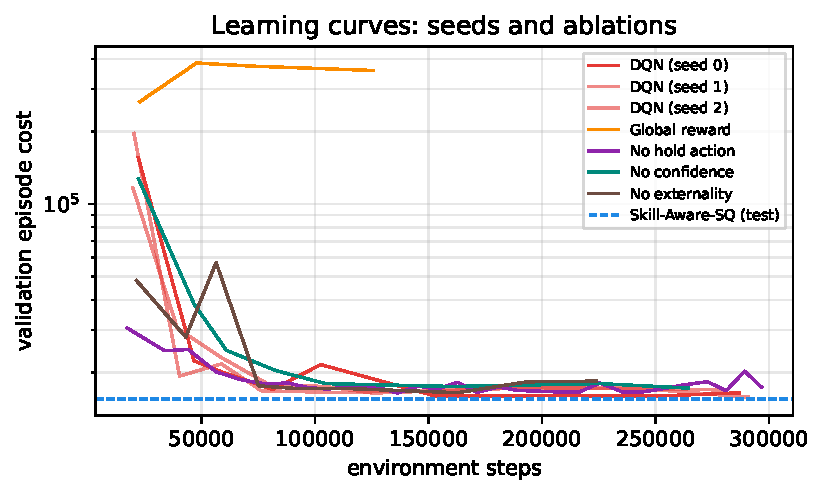
\includegraphics[width=\linewidth]{ablation_curves}
\caption{Validation cost during training: three seeds and ablations. The global-reward
DQN never learns; the dashed line is Skill-Aware-SQ.}
\label{fig:curves}
\end{figure}

\begin{figure}[t]
\centering
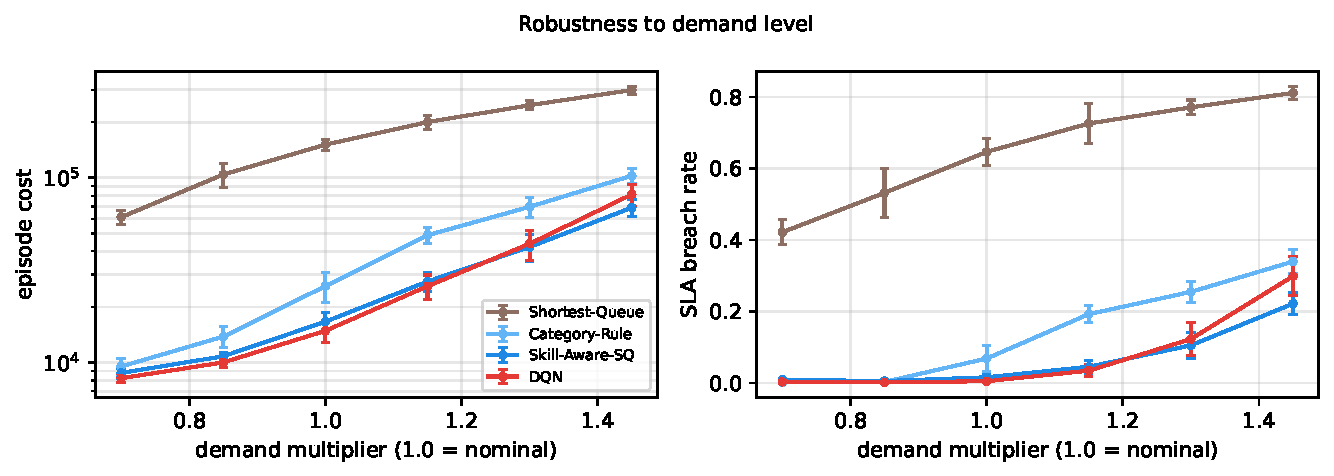
\includegraphics[width=\linewidth]{load_sweep}
\caption{Cost and SLA-breach rate vs.\ demand (10 shifts per point). The DQN is the cheapest
policy at every demand level.}
\label{fig:sweep}
\end{figure}

\begin{figure}[t]
\centering
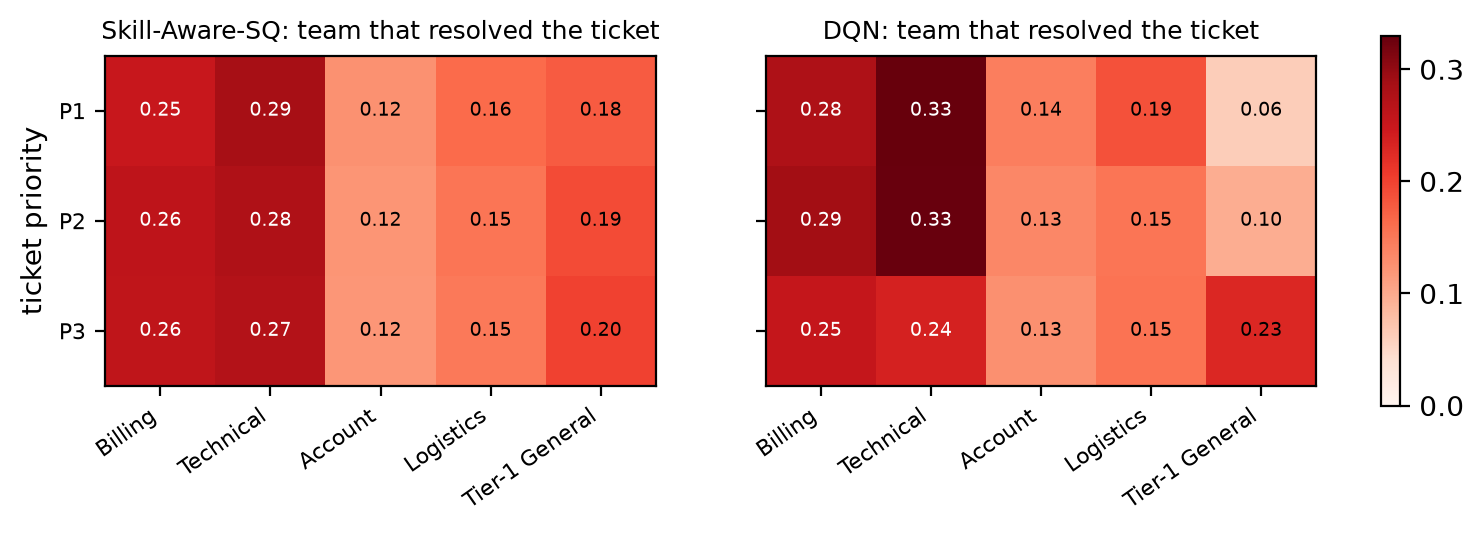
\includegraphics[width=\linewidth]{routing_heatmap}
\caption{Share of each priority's tickets resolved by each team.}
\label{fig:heat}
\end{figure}

\textbf{Headline} (Table~\ref{tab:main}). The DQN cuts operating cost by 88\% vs.\ Round-Robin,
90\% vs.\ Shortest-Queue, 46\% vs.\ Category-Rule and 9.3\% vs.\ Skill-Aware-SQ, which it beats
on 29/30 paired shifts (paired saving $1436\pm349$, $t{=}8.1$). SLA breaches fall
4$\times$ (1.3\%$\to$0.3\%), P1 breaches 2.7$\times$ (4.1\%$\to$1.5\%), mean resolution time from
17.0 to 15.2\,min. Across three training seeds the cost is $14{,}131\pm76$ (std).

\textbf{What was learned} (Fig.~\ref{fig:heat}). The agent discovered priority-aware use of the
slow generalist: it sends only 6\% of P1 tickets there (heuristic: 18\%) but 23\% of P3 tickets
(20\%), reserving fast specialists for urgent work -- a $c\mu$-like rule that was never
hand-coded. Its misroute rate is higher (0.24 vs 0.18 per ticket), but the extra penalties are
outweighed by shorter waits and fewer breaches.

\textbf{Ablations} (Fig.~\ref{fig:curves}; nominal / $1.45\times$ demand, 30 test shifts).
\emph{Global reward} (same DQN on the system-wide cost stream): cost 126{,}158, 56\% breaches --
credit assignment is essential. \emph{No confidence} (top-1 label only): $+3.4\%$ cost.
\emph{No externality}: $+3.1\%$ at nominal and $+9.3\%$ at $1.45\times$ (25\% vs 19\% breaches),
so the Pigouvian term matters under congestion. \emph{No hold}: $-2.5\%$ / $-4.0\%$, i.e.\ with
the fixes above the hold action is not needed; we keep it in the main agent for comparability.

\textbf{Robustness} (Fig.~\ref{fig:sweep}). The DQN is the cheapest policy at every demand
level from $0.7\times$ ($-8.5\%$ vs.\ Skill-Aware-SQ) to $1.45\times$ ($-3.7\%$). On the 30 test
shifts at $1.45\times$ all three seeds beat Skill-Aware-SQ (60.8k--62.6k vs.\ 64.2k) with at most
1.8 holds/ticket; before fixes (i) and (iii) and multi-load selection the agent was 18\% worse there.

\section{Discussion \& Limitations}
RL pays off where heuristics are blind: classifier confidence, urgency and heterogeneous service
rates. Its margin shrinks under extreme overload, where per-ticket credit assignment remains
partly selfish; better externality estimates or centralised critics are natural next steps. The
simulator's parameters are synthetic; with real logs they would be fit from ticket histories.

\footnotesize
\begin{thebibliography}{9}\setlength{\itemsep}{0pt}
\bibitem{mnih2015} V.~Mnih et al., ``Human-level control through deep reinforcement learning,'' \emph{Nature}, 518:529--533, 2015.
\bibitem{vanhasselt2016} H.~van Hasselt, A.~Guez, D.~Silver, ``Deep reinforcement learning with double Q-learning,'' \emph{AAAI}, 2016.
\bibitem{wang2016} Z.~Wang et al., ``Dueling network architectures for deep reinforcement learning,'' \emph{ICML}, 2016.
\bibitem{bradtke1995} S.~J.~Bradtke, M.~O.~Duff, ``Reinforcement learning methods for continuous-time Markov decision problems,'' \emph{NIPS}, 1995.
\bibitem{tang2019} X.~Tang et al., ``A deep value-network based approach for multi-driver order dispatching,'' \emph{KDD}, 2019.
\bibitem{roughgarden2002} T.~Roughgarden, \'E.~Tardos, ``How bad is selfish routing?,'' \emph{J. ACM}, 49(2):236--259, 2002.
\bibitem{sutton2018} R.~S.~Sutton, A.~G.~Barto, \emph{Reinforcement Learning: An Introduction}, 2nd ed., MIT Press, 2018.
\end{thebibliography}
\end{document}
